\section{Колористика в архитектуре Севера}

Проблема цветовых решений городского пространства исследовалась многими специалистами.
Так, в работах В.Ж. Елизарова, В.А. Глинкина, В.П. Белякова, А.В. Ефимова, Э.П. Путинцева рассматривались отдельные аспекты проблемы колористических решений,включая северные города.
В фундаментальных исследованиях А.В. Ефимова, где он ссылается на исследования Жана-Филиппа Ланкло, выявляются два противоположных подхода к колористическому формированию среды города.
Первый из них, исторический, заключается в интеграции архитектуры в природную стилистику окружения. Он берет свое начало с первых построек человека,
использования натуральных строительных материалов. Поэтому для такого подхода характерна монохромная или сдержанная цветовая гамма.
Второй подход, заключающийся в противопоставлении антропогенной среды природе, также находит отражение в мировой практике.
Для него в большей степени характерна полихромия, смелые цветовые решения и явный контраст с окружающей природой.
В качестве примера приводятся небольшие поселения на северных территориях Норвегии и Канады, где в условиях почти круглогодичного природного «цветового голодания» рождаются
яркие колористические решения в застройке \Code{[52]}.

Стоит отметить факт, основанный на наблюдениях: цвет играет важную роль для защиты от воздействия тепловой энергии солнца.
Так, в Туле в 1954 году был проведен эксперимент, в котором часть покрытия аэродромов была выполнена в белом цвете, часть в черном.
За лето глубина оттаивания грунта под черным покрытием составила 2,25 м, тогда как под белым – 1,65 м.
За счет отражающих свойств белого покрытия можно уменьшать воздействие на многолетнемерзлые грунты \Code{[17, с. 44]}.
Формирование единого похода к колористическому решению крупного города – задача на порядок более сложная, чем отдельного здания или маленького поселка,
так как происходит переход от масштаба одного здания к ансамблевому решению или колористическому объединению квартала, района или целого города.
В 2021 году Информационно-аналитическим центром Государственной комиссии по вопросам развития Арктики был опубликован проект «Дизайн-кода арктических поселений» .
Основная цель этого проекта – создание единых требований к оформлению северного города для формирования его уникального облика.
В нем очень подробно изучаются существующие элементы внешнего оформления на примере трех населенных пунктов: Апатиты, Полярный и Никель.
Далее выявляются удачные и неприемлемые решения по размещению вывесок, баннеров, орнаментов, информационных стендов, памятных табличек, элементов навигации и т.д.,
а также даются рекомендации. Данный подход используется с целью облагораживания среды городов, избавления от «замусоривания» разномастными элементами оформления,
что должно послужить на пользу развития городов. Одновременно с этим рассматриваются колористические решения фасадов,
вопросы использования суперграфики как попытки внести разнообразие в среду города.

На наш взгляд, данная рекомендация в «Дизайн-коде арктических поселений» оказывается спорной.
Она объяснима с точки зрения попытки создания гармоничного цветового решения в городе, однако несколько противоречит выводам,
сделанным многими специалистами на основании фундаментальных исследований за 30–40 лет до этого.
Учитывая то, что в рамках этого исследования нам необходимо сформулировать выводы и рекомендации,
то лучшим выходом будет собрать самое ценное из различных концепций и найти «золотую середину».
Нельзя игнорировать исследования, даже если они проведены более тридцати лет назад: их база не меняется,
глубокое исследование исторических мотивов и опыта предыдущих поколений может быть использовано и сейчас.
Одновременно с этим, современные исследования отличаются большей полнотой и актуальностью собранных данных.
Таким образом можно делать новые заключения, опираясь на все доступные данные и адаптируя их к современным реалиям.
В частности, компромиссом по колористике может быть решение по использованию теплых насыщенных оттенков вместо простых «баночных» цветов при окраске фасадов.
В таком случае даже насыщенные цветовые решения, основанные на контрасте, могут гармонично сочетаться с природным окружением и при этом продолжать выполнять практические функции.

Отдельный момент колористического подхода в попытке формирования уникальной среды – это использование стрит-арта на фасадах зданий.
Данный прием позволяет делать даже здания типовой застройки интересными, нетипичными, а также отражать идентичность места, связанную с национальными или культурными традициями (рис. 4).
Рекомендации, связанные с использованием данного вида оформления, связаны с его визуальным восприятием. Так как размеры таких изображений монументальны,
нужно заранее просчитывать точки и углы возможного обзора для реализации их максимального эффекта.
Также хотелось бы отметить, что в Мурманске можно наблюдать преимущественно геометрические и стилизованные примеры данного вида искусства,
тогда как в Якутске они тяготеют к национальным и природным мотивам, что говорит о различной истории и культурных особенностях этих городов.

\begin{figure}[h]
    \begin{center}
        \hfill
        \begin{minipage}[h]{0.42\linewidth}
            \center{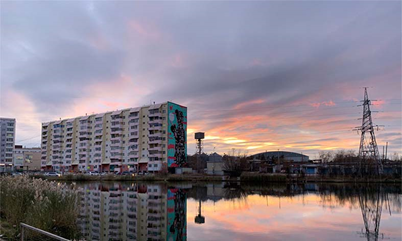
\includegraphics[height=1\linewidth]{assets/figures/st1_colouristic_yakutsk_01.png}} \\ а) 
        \end{minipage}
        \hfill
        \begin{minipage}[h]{0.42\linewidth}
            \center{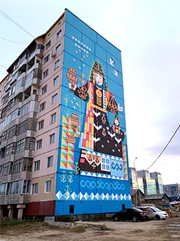
\includegraphics[height=1\linewidth]{assets/figures/st1_colouristic_yakutsk_02.png}} \\б)
        \end{minipage}
        \hfill
    \end{center}
    % \vfill
    \begin{center}
        \hfill
        \begin{minipage}[h]{0.3\linewidth}
        \center{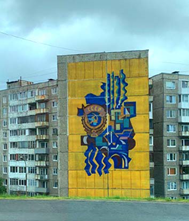
\includegraphics[height=1\linewidth]{assets/figures/st1_colouristic_murom_02.png}} \\ в)
        \end{minipage}
        \hfill
        \begin{minipage}[h]{0.3\linewidth}
        \center{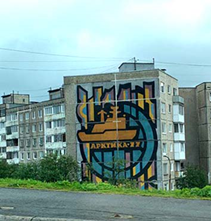
\includegraphics[height=1\linewidth]{assets/figures/st1_colouristic_murom_03.png}} \\ г)
        \end{minipage}
        \hfill
        \begin{minipage}[h]{0.3\linewidth}
        \center{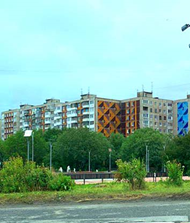
\includegraphics[height=1\linewidth]{assets/figures/st1_colouristic_murom_01.png}} \\ д)
        \end{minipage}
    \end{center}
    \caption{Примеры использования стрит-арта на фасадах зданий (мурал арт) в северных городах.
                Якутск: а) улица Лермонтова, д. 58/2; б) улица Лермонтова, д. 56;
                Мурманск: в) Кольский проспект, д. 142; г) Кольский проспект, д. 138, к. 1; д) улица Зои Космодемьянской, д. 32-36
                }
    \label{fig:st1coloristic_murals}
    \end{figure}